\documentclass[hyperref={unicode=true}]{beamer}
\usepackage[utf8]{inputenx}
\usepackage[russian]{babel}

\usepackage{multicol}

\usepackage[pgf]{dot2texi}
\usepackage{tikz}
\usetikzlibrary{shapes, arrows}

\usepackage{listings}
\usepackage{graphicx}

\usepackage{comment}

\title{Лекция 13. Моделирование Java-программ}
\author{}
\date{}

\usetheme{Warsaw}

\AtBeginSection[] {
	\begin{frame}{Содержание}
		\tableofcontents[currentsection]
	\end{frame}
}
%\overfullrule=5pt

\begin{document}
	\begin{frame}{}
		\titlepage
	\end{frame}

    \begin{frame}{Цель лекции}
    Обсудить моделирование Java-программы (в
    первую очередь, модель памяти), потому что
    AstraVer работает на той же аксиоматизации
    \end{frame}

    \section{Почему Java?}

    \begin{frame}{Jessie и Krakatoa}
    \begin{itemize}
    \item
    AstraVer -- наследник инструмента Jessie.
    Jessie моделирует Си-программу на Why3
    и использует общую модель памяти с
    инструментом Krakatoa, который моделирует
    Java-программы.
    \item
    Krakatoa должен был доказывать правильность
    программ для JavaCard. После окончания
    проекта инструмент не развивается.
    \end{itemize}
    \end{frame}

    \begin{frame}{Картинка с семейством инструментов}
    \begin{figure}
    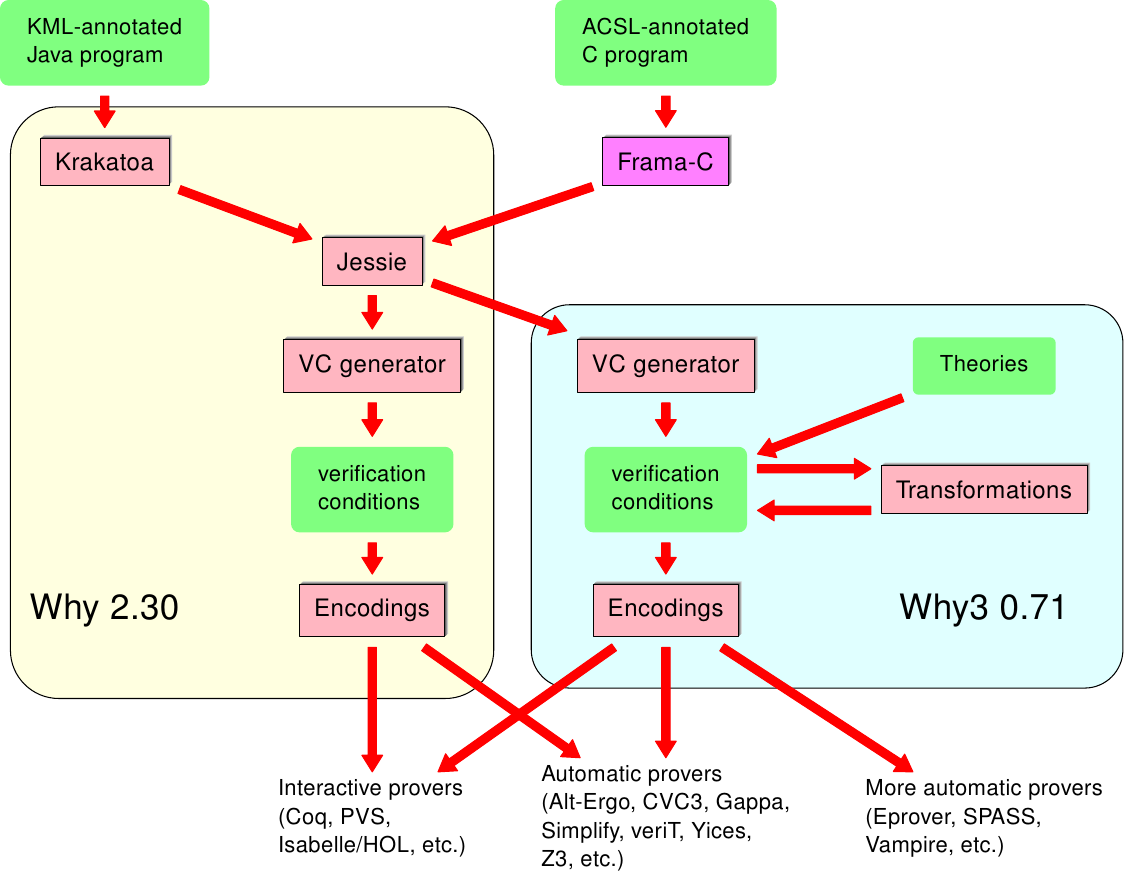
\includegraphics[height=0.8\textheight]{why_frama_c2-mps.png}
    \end{figure}
    \end{frame}

    \begin{frame}{Почему для Си модель памяти языка Java?}
    \begin{itemize}
    \item
    Много похожего, хотя есть и отличия
    \item
    Можно переиспользовать готовые инструменты, модели,
    модули для Java, раз они уже были к моменту создания Jessie
    \end{itemize}
    \end{frame}

    \section{Особенности Javа-программ}

    \begin{frame}{Чего нет в Си?}
    \begin{itemize}
    \item
    Инкапсуляция (классы, поля, методы)
    \item
    Наследование
    \item
    Полиморфизм (виртуальные методы)
    \item
    Специфичные возможности: исключения, instanceof
    и приведения типа, оператор new, интерфейсы и т.п.
    \item
    Ссылочная модель памяти
    \end{itemize}
    \end{frame}

    \begin{frame}{Модель требований}
    \begin{itemize}
    \item
    Язык спецификации ООП-программы -- это
    зыбкая область. Много вопросов, нет решений,
    принятых всем сообществом программистов.
    \item
    Основная проблема спецификаций ООП-программы --
    большое число требований к коду, потому что
    это ООП-код (с классами, с интерфейсами).
    \item
    Решение №1: в языке спецификации уже есть
    бОльшая часть моделей типовых требований; какие
    плюсы и минусы?
    \item
    Решение №2: язык спецификации содержит небольшое
    число возможностей и средства определения новых;
    какие плюсы и минусы?
    \end{itemize}
    \end{frame}

    \begin{frame}{Модель требований у нас}
    \begin{itemize}
    \item
    Ввиду отсутствия хороших решений, мы не будем
    касаться темы языка спецификации ООП-программ
    \item
    Будем предполагать, что каждый метод каждого
    класса снабжен парой из предусловия и постусловия
    \end{itemize}
    \end{frame}

    \begin{frame}{Дополнение модели требований из-за исключений}
    \begin{itemize}
    \item
    Т.к. метод может завершиться из-за необработанного
    исключения, то надо предусмотреть постусловие
    <<для завершения по исключению>>
    \item
    Это как будто мы вводим в блок-схему новый вид операторов
    (HALT-RAISES): оператор завершения блок-схемы из-за исключения
    \item
    Частичная корректность:
        \begin{enumerate}
        \item
        если вычисление завершилось на
        операторе HALT-RAISES, то должно быть выполнено постусловие
        <<для завершения по исключению>>
        \item
        если вычисление завершилось на операторе HALT,
        то должно быть выполнено обычное постусловие
        \end{enumerate}
    \end{itemize}
    \end{frame}

    \section{Построение модели Java-программы}

    \begin{frame}{Что надо уметь моделировать?}
    \begin{itemize}
    \item
    обращение к полю (возможно, поле находится в классе-предке)
        \begin{itemize}
        \item
        надо собрать поля из всех классов-предков
        \end{itemize}
    \item
    вызов виртуального метода
        \begin{itemize}
        \item
        предполагаем, что мы верифицируем фиксированную программу,
        с фиксированным набором классов и наследования; значит,
        можно перебрать динамические типы объекта в виде условного
        выбора и для каждого типа вызвать метод из нужного класса
        \item
        нужно поддерживать динамические типы для каждого указателя
        \end{itemize}
    \item
    генерация исключения и обработка исключения в разных методах
        \begin{itemize}
        \item
        используем встроенные возможности Why3 по поддержке
        исключений
        \end{itemize}
    \end{itemize}
    \end{frame}

    \begin{frame}{Что надо уметь моделировать?}
    \begin{itemize}
    \item
    оператор new
        \begin{itemize}
        \item
        добавляем новый блок в alloc\_table и вызываем
        метод-конструктор
        \end{itemize}
    \item
    оператор instanceof
        \begin{itemize}
        \item
        динамические типы уже поддерживаются, остается добавить
        соотношения на типах, что они находятся в иерархии наследования
        \end{itemize}
    \item
    приведение типов ссылок
        \begin{itemize}
        \item
        это всего лишь проверка динамического типа, сама ссылка
        и объект не меняются
        \end{itemize}
    \end{itemize}
    \end{frame}

    \begin{frame}{Упражнение}
    \begin{itemize}
    \item
    Попробуйте применить эти идеи для доказательства
    полной корректности кода классов Account, CreditAccount
    и Prog (который тестирует предыдущие классы)
    \end{itemize}
    \end{frame}

    \begin{frame}{Выводы}
    \begin{itemize}
    \item
    Нужно добавлять поля класса-предка в класс-потомок
    \item
    Нужно моделировать иерархии классов по наследованию
    (tag -- элемент иерархии, на тэгах определено отношение
    subtag, в иерархии есть нижний тип bottomtag).
    \item
    Модель памяти (из memory и alloc\_table) нужно
    дополнить таблицей с динамическими типами переменных
    (tag\_table)
    \item
    Тип переменной memory должен типизироваться типом bottomtag,
    т.к. в этой переменной должны быть указатели разных
    типов в рамках одной иерархии (т.к. типы указатели на класс-предок
    и на класс-потомок не отличаются, иначе было бы сложно
    делать приведение типов и обращение к полю класса-предка как
    приведения к нужному типу-предку и обращению к memory с его типом)
    \end{itemize}
    \end{frame}
\end{document}
